\newpage
{\bfseries МРНТИ 31. 21.19}

\sectionwithauthors{С.Д. Фазылов, Ж.Б. Сатпаева, О.А. Нуркенов, Р.Е. Бакирова, А.К. Свидерский, А.Ж. Мендибаева}{ПОЛУЧЕНИЕ ВОДОРАСТВОРИМЫХ КОМПЛЕКСОВ ВКЛЮЧЕНИЙ ГИДРАЗИДОВ \emph{о-} И \emph{п}-ГИДРОКСИБЕНЗОЙНЫХ КИСЛОТ И ИХ
ГИДРАЗОНОВЫХ ПРОИЗВОДНЫХ}

\begin{center}
{\bfseries \textsuperscript{1}С.Д. Фазылов, \textsuperscript{2}Ж.Б. Сатпаева, \textsuperscript{1}О.А. Нуркенов, \textsuperscript{3}Р.Е. Бакирова, \textsuperscript{4}А.К. Свидерский, \textsuperscript{1}А.Ж. Мендибаева}

\textsuperscript{1}Институт органического синтеза и углехимии РК,
Караганда, Казахстан,

\textsuperscript{2}НАО «Карагандинский университет им. Е.А. Букетова»,
Караганда, Казахстан,

\textsuperscript{3}Медицинский университет Караганды, Караганда,
Казахстан,

\textsuperscript{4} Жезказганский университет им. О.А. Байконурова,
Жезказган, Казахстан

Корреспондент-автор: iosu8990@mail.ru
\end{center}

В статье представлены результаты исследований по получению
водорастворимых комплексов биологически активных гидразидов и
гидразонов, получаемых на основе производных \emph{о-} и
\emph{п}- гидроксибензойных кислот. Гидразоны находят широкое применение
медицине в качестве противотуберкулезных антибактериальных и
противовоспалительных препаратов, антисептиков, консервантов и других
биоактивных субстратов. Для большинства из них характерно низкая
растворимость в воде, что ограничивает дальнейшее их изучение на
биологическую активность. В статье показано, что гидразиды \emph{о}- и
\emph{п}- гидроксибензойных кислот и их гидразоновые производные могут
образовывать различные комплексы включений с природными
макромолекулярными биополимерами. Рассмотренные в статье новые
гидразоновые продукты, способны растворяться в воде, а также
образовывать устойчивые водные дисперсии. Получение водорастворимых
комплексов указанных соединений могут привести к повышению их
биологической доступности, что соответственно позволит значительно
сократить их терапевтическую концентрацию. Показано, что комплексы между
молекулами биополимера и субстрата являются достаточно стабильными. При
этом молекула комплексообразователя будет способствовать защите молекулы
субстрата от взаимодействия с различными высоко реакционноспособными
молекулами, снижая скорость окисления, гидролиза и/или деструкции, а
также вероятность стерических перегруппировок и рацемизации. Описанные в
работе новые комплексы включений гидразидов и гидразонов \emph{о-} и
\emph{п- }гидроксибензойных кислот охарактеризованы с помощью ИК- и
ЯМР-\textsuperscript{1}Н спектроскопии, дифференциальной сканирующей
термогравиметрии и сканирующего электронного микроскопа.

{\bfseries Ключевые слова:} \emph{о}- и \emph{п}- гидроксибензойные
кислоты, гидразид, гидразон, макромолекулы, комплекс включения,
дифференциальная термогравиметрия.

\sectionheading{ГИДРОКСИБЕНЗОЙ ҚЫШҚЫЛ ГИДРАЗИДТЕРІ МЕН ОЛАРДЫҢ ГИДРАЗОНДЫ
ТУЫНДЫЛАРЫНЫҢ СУДА ЕРИТІН КЕШЕНДЕРІН АЛУ}

\begin{center}
{\bfseries \textsuperscript{1}С.Д. Фазылов, \textsuperscript{2}Ж.Б.
Сәтпаева, \textsuperscript{1}О.А. Нүркенов, \textsuperscript{3}Р.Е.
Бәкірова,}

{\bfseries \textsuperscript{4}А.К. Свидерский, \textsuperscript{1}Ә.Ж.
Мендібаева}

\textsuperscript{1}ҚР Органикалық синтез және көмірхимиясы институты,
Қарағанды, Қазақстан,

\textsuperscript{2}КЕАҚ «Е.А. Букетов атындағы Қарағанды университеті»,
Қарағанды, Қазақстан,

\textsuperscript{3}Қарағанды медицина университеті, Қарағанды,
Қазақстан,

\textsuperscript{4} Ө.А.Байқоңыров атындағы Жезқазған университеті,
Жезқазған, Қазақстан,

e-mail: iosu8990@mail.ru
\end{center}

Мақалада \emph{о}- және \emph{п}-гидроксибензой қышқылдары негізінде
алынатын биологиялық белсенді гидразидтер мен гидразондардың суда еритін
кешендерін алу бойынша зерттеу нәтижелері ұсынылған. Гидразондар
медицинада туберкулезге, бактерияға және қабынуға қарсы препараттар,
антисептиктер, консерванттар және басқа биоактивті субстраттар ретінде
кеңінен қолданылады. Олардың көпшілігі суда төмен ерігіштігімен
сипатталады, бұл олардың әрі қарай биологиялық белсенділігін зерттеуге
шектеу қояды. Мақалада \emph{о-} және \emph{п-}гидроксибензой қышқыл
гидразидтері мен олардың гидразон туындылары табиғи макромолекулалық
биополимерлермен әр түрлі қосу кешендерін құра алатыны көрсетілген.
Мақалада талқыланған жаңа гидразон өнімдері суда ериді, сонымен қатар
тұрақты сулы дисперсиялар түзеді. Осы қосылыстардың суда еритін
кешендерін алу олардың биологиялық қолжетімділігін жоғарылауына әкелуі
мүмкін, бұл тиісінше олардың емдік концентрациясын төмендетеді.
Биополимер мен субстрат молекулалары арасындағы комплекстердің
айтарлықтай тұрақты болатыны дәлелденді. Бұл жағдайда комплекс түзуші
молекула субстрат молекуласы әр түрлі жоғары реактивті молекулалармен
әрекеттесуден қорғауға көмектесіп, тотығу, гидролиз және/немесе жойылу
жылдамдығын, сондай-ақ кеңістіктік қайта құрылымдау мен рацемизация
ықтималдығын төмендетеді. Жұмыста сипатталған \emph{о}- және
\emph{п}-гидроксибензой қышқылдар гидразидтер мен гидразондарының жаңа
комплексті кешендері ИҚ- мен \textsuperscript{1}Н-ЯМР спектроскопиясы,
дифференциалды сканерлеуші термогравиметрия мен сканерлеуші электронды
микроскоп арқылы сипатталды.

{\bfseries Түйін сөздер:} \emph{о}- және \emph{п}-гидроксибензой
қышқылдары, гидразид, гидразон, макромолекулалар, қосылу кешендері,
дифференциальды термогравиметрия.

\sectionheading{PREPARATION OF WATER-SOLUBLE COMPLEXES OF INCLUSIONS HYDRAZIDES
OF \emph{o}- AND \emph{p}-HYDROXYBENZOIC ACIDS AND THEIR HYDRAZONE
DERIVATIVES}

\begin{center}
{\bfseries \textsuperscript{1}S.D. Fazylov, \textsuperscript{2}Zh.B.
Satpaeva, \textsuperscript{1}O.A. Nurkenov, \textsuperscript{3}R.Е.
Bakirova,}

{\bfseries \textsuperscript{4}А.К. Sviderskyi, \textsuperscript{1}A.Zh.
Mendibayeva}

\textsuperscript{1}Institute of Organic Synthesis and Coal Chemistry,
Karaganda, Kazakhstan,

\textsuperscript{2}Karaganda Buketov University, Karaganda, Kazakhstan,

\textsuperscript{3} Karaganda Medical University, Karaganda, Kazakhstan,

\textsuperscript{4} Zhezkazgan University, Zhezkazgan, Казахстан,

e-mail: iosu8990@mail.ru
\end{center}

The article presents the results of studies on obtaining water-soluble
complexes of biologically active hydrazides and hydrazones derived from
derivatives of \emph{o-} and \emph{p-}hydroxybenzoic acids. Hydrazones
are widely used in medicine as antitubercular antibacterial and
anti-inflammatory drugs, antiseptics, preservatives and other bioactive
substrates. Most of them are characterized by low solubility in water,
which limits their further study for biological activity. The paper
shows that hydrazides of \emph{o-} and \emph{p-}hydroxybenzoic acids and
their hydrazone derivatives can form various inclusion complexes with
natural macromolecular biopolymers. The new hydrazone products
considered in this article are able to dissolve in water and also form
stable aqueous dispersions. Obtaining water-soluble complexes of these
compounds can lead to an increase in their bioavailability, which,
accordingly, will allow to significantly reduce their therapeutic
concentration. Complexes between biopolymer and substrate molecules have
been shown to be quite stable. In this case, the host complexing
molecule will contribute to the protection of the substrate molecule
from interaction with various highly reactive molecules, reducing the
rate of oxidation, hydrolysis and/or degradation, as well as the
probability of steric rearrangements and racemization. The new inclusion
complexes of hydrazides and hydrazones of \emph{o-} and
\emph{p-}hydroxybenzoic acids described in this work have been
characterized by IR and NMR-1H spectroscopy, differential scanning
thermogravimetry and scanning electron microscope.

{\bfseries Keywords:} \emph{o-} and \emph{p-}hydroxybenzoic acids,
hydrazide, hydrazone, macromolecules, inclusion complex, differential
thermogravimetry.

\begin{multicols}{2}
{\bfseries Введение.} Гидразиды и гидразоны, полученные на основе
производных \emph{о-} и \emph{п-}гидроксибензойных кислот находят
широкое применение медицине в качестве противотуберкулезных
антибактериальных и противовоспалительных препаратов, антисептиков
{[}1{]}, консервантов {[}2{]} и других биоактивных субстратов {[}3{]}.
Однако для большинства из них характерно низкая растворимость в воде,
что ограничивает дальнейшее их изучение на биологическую активность, в
частности, такое свойство характерно для многих производных гидразидов
\emph{о-} и \emph{п}-гидроксибензойных кислот. В настоящее время в
фармакологии разработаны и используются различные пути повышения
растворимости биоактивных веществ в полярных растворителях с
использованием специальных макромолекулярных биополимеров -
краун-эфиров, криптандов, циклофанов, каликсаренов и полисахаридов как
комплексообразователей {[}4{]}. Вышеуказанные биополимеры имеют
гидрофобную внутреннюю полость и гидрофильную внешнюю оболочку.
Получением комплекса включения можно увеличить также стабильность
низкомолекулярных веществ, чувствительных к действию света и кислорода
воздуха, увеличить их растворимость в воде, биодоступность, а также
снизить токсичность.

Комплексы между молекулами биополимера и субстрата, формирующиеся под
действием нековалентных сил (ван-дер-ваальсовых, гидрофобных и т.п.),
являются достаточно стабильными. При этом молекула
комплексообразователя-хозяина будет способствовать защите молекулы
субстрата от взаимодействия с различными высоко реакционноспособными
молекулами, снижая скорость окисления, гидролиза и/или ферментативной
деструкции, вероятность стерических перегруппировок и рацемизации
{[}4{]}. К одним из таких перспективных природных комплексообразователей
можно отнести природные олигосахариды (циклодекстрины), получаемые
ферментативной деструкцией картофельного крахмала {[}5{]}. Они имеют
молекулу в форме усеченного конуса с внутренними (Н\textsubscript{3} и
Н\textsubscript{5}) и внешними (Н\textsubscript{2} и Н\textsubscript{4})
протонами. Такая структура молекулы циклодекстрина обеспечивает
возможность вхождения активной субстанции в полость рецептора в
результате гидрофобных взаимодействий между БАВ и
комплексообразователем. Синтезированные нами новые гидразиды и гидразоны
(3-5) \emph{о}- и \emph{п}-гидрокисибензойных кислот {[}6{]} мало
растворимы в воде. В настоящей работе нами представлены результаты
исследования по получению водорастворимых комплексов включений новых
синтезированных нами гидразидов и их гидразоновых производных {[}6{]} с
природным олигомером.

{\bfseries Материалы и методы.} В качестве субстратов для получения
комплексов включений были использованы синтезированные нами {[}6{]}
гидразиды (1 и 2), а также их гидразоновые производные:
N-(4-(диэтиламино)-2-гидроксибензилиден)-2-гидроксибензогидразид (3),
N-(4-(диэтиламино)-2-гидроксибензилиден)-4-гидроксибензогидразид (4),
N-(2-хлор-6-фторбензилиден)-4-гидроксибензогидразид (5). В качестве
комплексообразователя был выбран β-циклодекстрин производства ``Fluka''
(США)(чистота 99\%). Все выше указанные вещества, при биоскрининге
показали умеренно-выраженную антимикробную активность и
характеризовались слабым антирадикальным эффектом {[}6{]}, а также
обладали низкой водорастворимостью {[}7-8{]}.

Получение комплексов соединений (6-10) с полисахаридом осуществлялось в
водно-спиртовой среде. К концентрированному раствору гидразида \emph{о-}
или \emph{п-}гидроксибензойных кислот (1, 2) в этаноле в мольном
соотношении 1:1 по каплям вносили насыщенный раствор β-циклодекстрина
(ЦД) в воде при температуре 80-90°С. Аналогично проводилось получение
комплексов гидразидов и гидразонов (8-10) с полисахараридом в
соотношении 1:2 (рисунок 1).
\end{multicols}

\begin{figure}[H]
	\centering
	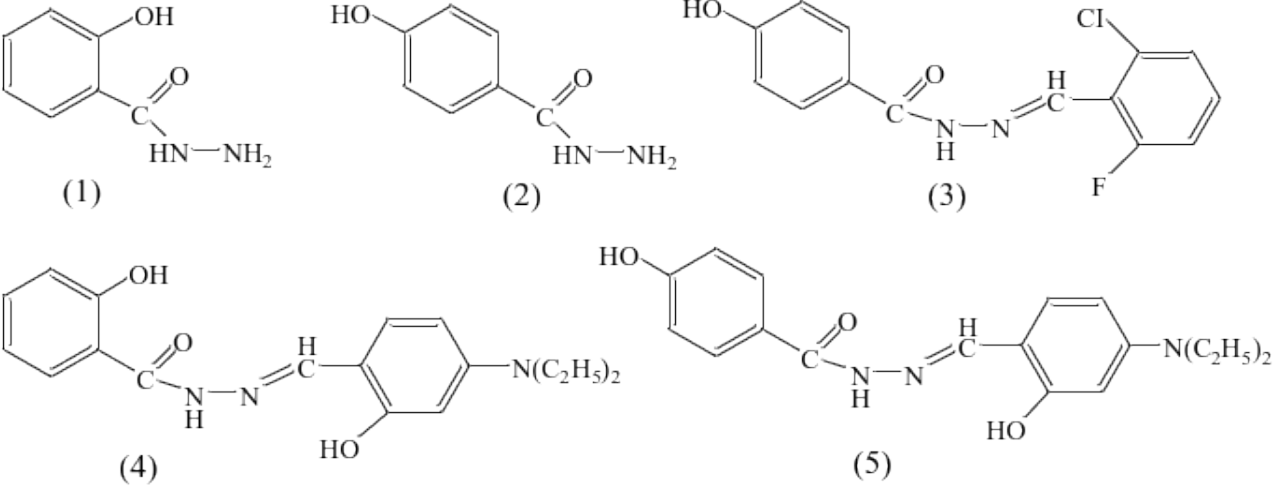
\includegraphics[width=0.9\textwidth]{assets/43.1}
	\caption*{}
\end{figure}

\begin{figure}[H]
	\centering
	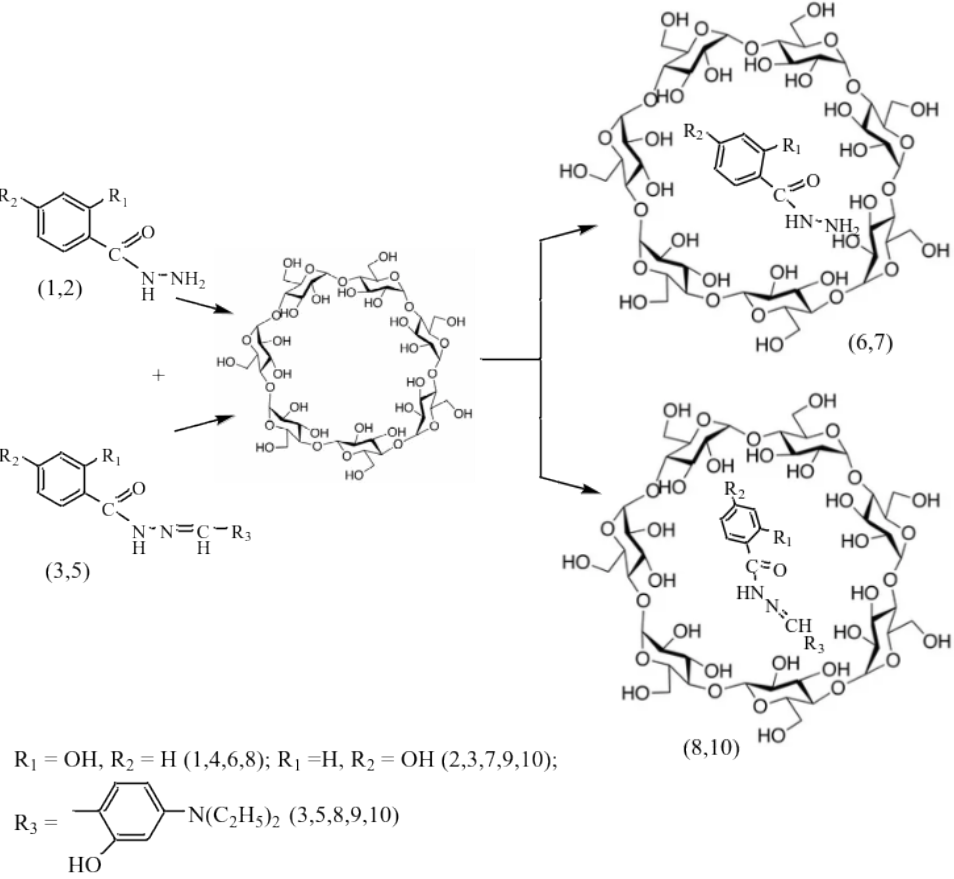
\includegraphics[width=0.85\textwidth]{assets/43.2}
	\caption*{Рис. 1 -- Схема синтеза комплексов включений соединений (6-10)}
\end{figure}

\begin{multicols}{2}
Комплексы включения гидразидов (1,2) и гидразонов (3-5) с ЦД-ном, а
также их комплексов (6-10) получали в виде кристаллических порошков
белого цвета с выходами 80-85\%. Конечные продукты были высушены в
сушильном шкафу при температуре 50±1°С. Полученные водорастворимые
комплексы включения гидразидов и их гидразоновые производные с ЦД-ном
(6-10) образуют устойчивые водные дисперсии, что приводит к повышению их
биологической доступности, тем самым сокращая их терапевтическую дозовую
концентрацию.

ИК спектры исходных и конечных продуктов регистрировали на спектрометре
с Фурье-преобразователем FSM 1201 по волновому числу в диапазоне от 4000
до 500 см\textsuperscript{-1} в таблетках с KBr. Спектры ЯМР
\textsuperscript{1}Н соединений снимали на спектрометре JNM-ECA Jeol 400
(частота 399.78 МГц) с использованием растворителей
ДМСО-d\textsubscript{6} и CDCl\textsubscript{3}. Химические сдвиги
измеряли относительно сигналов остаточных протонов или атомов углерода
дейтерированного растворителя. Температуры плавления определяли на
приборе «SMP10». Термогравиметрический (ТГ), дифференциальный
термический (ДТГ) и дифференциально-сканирующий калориметрический (ДСК)
анализ проводили на оборудовании ДТА/ДСК (Labsys EVO, Setaram, Франция)
в динамическом режиме в диапазоне температур 30-500°С при скорости
нагрева 100°С/мин в атмосфере азота и воздуха.

{\bfseries Результаты и обсуждение.} На рисунке 2 приведены ИК спектры ЦД
(а), физической смеси ЦД с (6) (б) и комплекса включения (6) (в).
\end{multicols}

\begin{figure}[H]
	\centering
	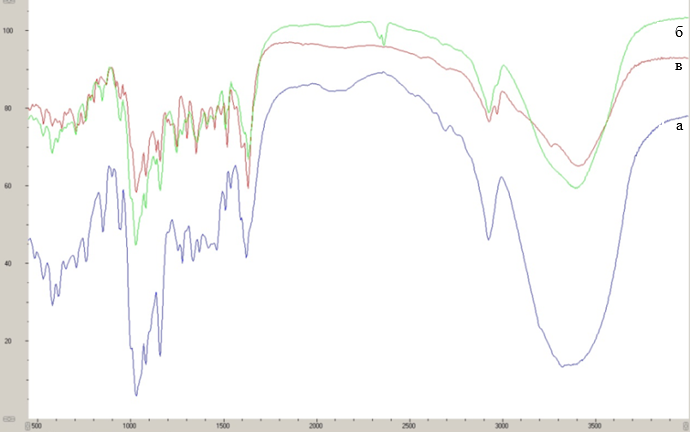
\includegraphics[width=0.7\textwidth]{assets/44}
	\caption*{Рис. 2 -- ИК спектр ЦД (а), физической смеси ЦД и субстрата (б), клатратного комплекса ЦД:(6) (в), соотношение (1:1)}
\end{figure}

\begin{multicols}{2}
В ИК спектре полученного комплекса (6) ОН-группы ЦД проявляются широкой
характерной полосой в области 3310-3320 см\textsuperscript{-1},
колебания связи С-Н прописываются в областях 2900-2910 и 887-892
см\textsuperscript{-1}. Следует отметить, что в ИК спектрах всех
комплексов включений (6-10) основные характерные полосы поглощения
субстратов (1-5) не проявляются, так как это можно объяснить эффектом
экранирования широкими полосами поглощения функциональных групп ЦД.
Однако, в спектрах наблюдаются смещение характерных полос поглощения
комплексообразователя (молекулы полисахарида).

В таблице 1 приведены значения химического сдвигов Δδ протонов
комплексообразователя в ЯМР-\textsuperscript{1}Н спектрах ЦД и его
комплексе включения с продуктом (6) (2:1) в свободном состоянии
δ\textsubscript{0}, м.д.) и в составе комплекса (δ, м.д.)
\end{multicols}

\begin{table}[H]
\centering
\caption*{Таблица 1 -- Значения химического сдвигов Δδ протонов в ЯМР-\textsuperscript{1}Н спектрах ЦД и его комплексе включения с продуктом (6) (2:1) в свободном состоянии (δ\textsubscript{0}, м.д.) и в составе комплекса (δ, м.д.)}
\begin{tabular}{|l|l|l|l|}
\hline
\multirow{2}{*}{Протон} & δ0, м.д.  (ЦД) & δ, м.д.   (ЦД:(6)) & Δδ (δ – δ0), м.д. \\ \cline{2-4} 
 & δ(1Н) & δ(1Н) & δ(1Н) \\ \hline
H1 & 4.77 & 4.76 & -0.01 \\ \hline
H2 & 3.26 & 3.28 & -0.02 \\ \hline
H3 & 3.43 & 3.35 & -0.08 \\ \hline
H4 & 3.27 & 3.26 & 0.01 \\ \hline
H5 & 3.43 & 3.37 & -0.06 \\ \hline
H6 & 3.58 & 3.59 & 0.01 \\ \hline
\end{tabular}
\end{table}

\begin{figure}[H]
    \centering
    \begin{subfigure}[b]{0.32\textwidth}
        \centering
        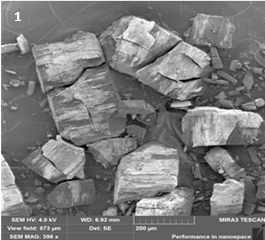
\includegraphics[height=0.9\textwidth]{assets/45}
    \end{subfigure}
    \hfill
    \begin{subfigure}[b]{0.32\textwidth}
        \centering
        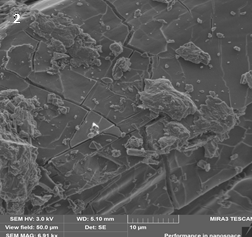
\includegraphics[height=0.9\textwidth]{assets/46}
    \end{subfigure}
    \begin{subfigure}[b]{0.32\textwidth}
        \centering
        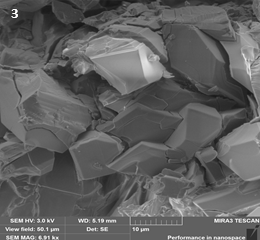
\includegraphics[height=0.9\textwidth]{assets/47}
    \end{subfigure}
\end{figure}

\begin{figure}[H]
    \centering
    \begin{subfigure}[b]{0.32\textwidth}
        \centering
        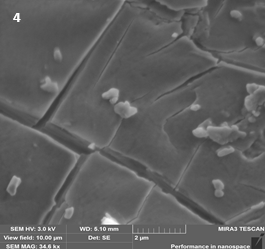
\includegraphics[height=0.9\textwidth]{assets/48}
    \end{subfigure}
    \hfill
    \begin{subfigure}[b]{0.32\textwidth}
        \centering
        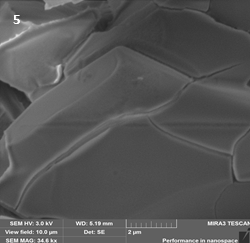
\includegraphics[height=0.9\textwidth]{assets/49}
    \end{subfigure}
    \begin{subfigure}[b]{0.32\textwidth}
        \centering
        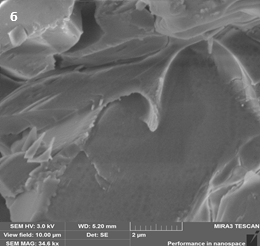
\includegraphics[height=0.9\textwidth]{assets/50}
    \end{subfigure}
    \caption*{Рис. 3 - Электронные микрофотографии ЦД (снимки 1, 2),
    физической смеси ЦД с (6) (снимки 3,4) и комплекса ЦД:(6) (2:1) (снимки
    при различных увеличениях)}
\end{figure}

\begin{multicols}{2}
На основании приведенных в таблице 1 данных можно отметить, что
наибольшее смещение испытывают протоны внутренней сферы полисахарида --
Н3 и Н5. Эти данные свидетельствуют в пользу образования внутреннего
комплекса β-ЦД с (6) {[}9-12{]}.

На рисунке 3 показаны микрофотографии кристалликов комплексов, снятых
при различных увеличениях, на сканирующем электронном микроскопе, СЭМ -
β-ЦД, физической смеси ЦД и вещества (6) и комплекса включения ЦД:(6)
(2:1). Снимки (1-6) были сделаны при различных ускоряющих напряжениях.
На многократно увеличенных снимках комплексов наблюдается резкое
изменение морфологии и формы кристаллов: кристаллические формы частиц
клатратов имеют более сглаженный вид (возможно, из-за пленкообразования
(снимки 5 и 6) при SEM MAG 69,2kx). Изменения морфологии поверхности
кристаллов при комплексообразовании субстрата с молекулой полисахарида
являются одним из доказательств образования комплексов включений.
\end{multicols}

\begin{figure}[H]
	\centering
	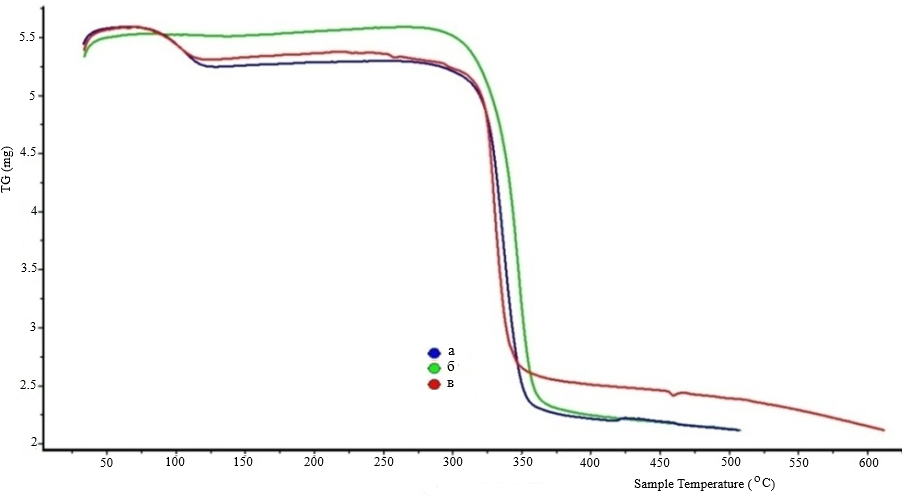
\includegraphics[width=0.8\textwidth]{assets/51}
	\caption*{Рис. 4 - Термогравиметрические кривые циклодекстрина (а), продукта (6) и комплекса включения ЦД:(6)}
\end{figure}

\begin{figure}[H]
	\centering
	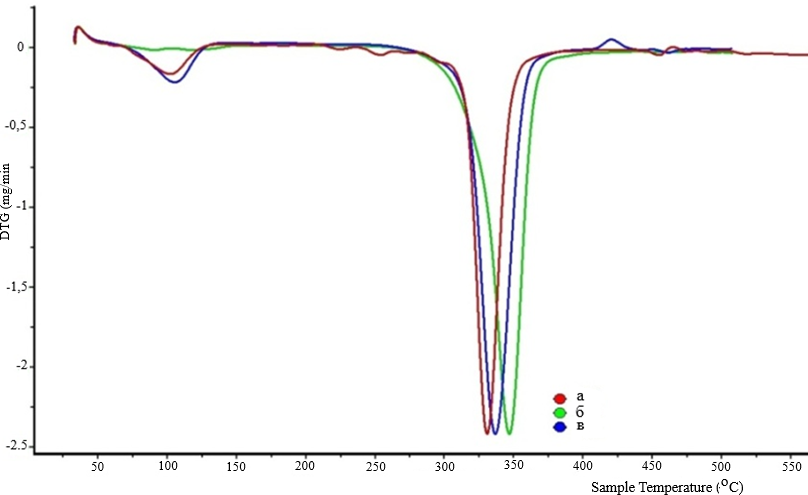
\includegraphics[width=0.8\textwidth]{assets/52}
	\caption*{Рис. 5 -- Дифференциальная сканирующая калориметрия комплекса включения ЦД:(6) (а), физической смеси ЦД:(6) (б) (соотношение (1:1) и циклодекстрина (в)}
\end{figure}

\begin{multicols}{2}
Термическую стабильность полученных комплексов включения гидразидов и их
гидразоновых производных при комплексообразовании с ЦД изучали с помощью
диференциального термического анализа (ДТА). С помошью метода
дифференциальной сканирующей калориметрии можно установить зависимость
изменение массы синтезированных супрамолекулярных комплексов включения
от температуры (термогравиметрическая кривая) и по ее пику точно
определить максимальную скорость горения комплекса {[}13{]}.

На рисунках 4 и 5 приведены TГ/ДТА кривые ЦД и физической смеси ЦД с (6)
и комплекса включения ЦД:(6). Согласно данным TГ в интервале температур
от 32,8°С до 320°С циклодекстриновый комплекс включения ЦД:(6) не
претерпевает превращений, приводящих к изменению его массы {[}14,15{]}.
Основное количество летучих компонентов выделилось при 330°С-370°С. В
этом интервале происходит интенсивная убыль массы комплекса, о чем
свидетельствует ход термогравиметрической кривой. Процесс деструкции
практический полностью завершается при температуре 380°С.

Синтезированные комплексы включения содержали воду, которому
свидетельствуют эндотермический пик дегидратации в диапазоне 50-125°С,
это является переходом ЦД в безводную форму в результате испарения воды
{[}14,15{]}. Процесс термодеструкции ЦД начинается с 300°С, в области
температур 329-348°С происходит термодеструкция комплекса включения, что
свидетельствует о повышении термостабильности ЦД при включении в его
полость биологически активного компонента (6). На кривой скорости потери
массы в интервале температур 32°С-270°С не наблюдается изменение
скорости. Начиная с 310°С наблюдается резкое увеличение скорости и
достигает своего пика при ≈ 340°С, значение скорости при данной
температуре составляет 1,7 мг/мин. Далее идет постепенное уменьшение, и
при 380°С скорость стабилизируется. На кривой ДСК при температуре 329°С
(9), 335°С (8), 348\textsuperscript{0}С (10) наблюдается эндотермический
пик, обусловленный плавлением, при этом масса вещества не меняется,
далее при температуре ≈ 370°С присутствует экзотермический эффект,
которое объясняется разложением образца с выделением летучих продуктов и
потерей массы.

{\bfseries Выводы.} В химической фармакологии используются различные пути
повышения растворимости биоактивных веществ с использованием специальных
макромолекулярных биополимеров - краун-эфиров, криптандов, циклофанов,
каликсаренов, хитазана и полисахаридов как комплексообразователей.
Получением комплексов включения можно увеличить растворимость и
стабильность низкомолекулярных веществ. Гидразиды \emph{о}- и \emph{п}-
гидроксибензойных кислот и их гидразоновые производные могут
образовывать различные комплексы включений с макромолекулярными
биополимерами. Полученные продукты образуют смесь, способных
растворяться в воде или образовывать устойчивые водные дисперсии.
Получение водорастворимых комплексов указанных соединений должно
привести к повышению их биологической доступности, что соответственно
позволит значительно сократить их терапевтическую концентрацию. Данные
физико-химических методов исследований (ИК-, ЯМР \textsuperscript{1}Н
спектры, ДТГ, СЭМ) могут быть использованы при анализе полученных
комплексов включений биоактивных веществ.

\emph{{\bfseries Финансирование:} Научно-исследовательская работа
осуществлена в рамках ГФ АР14869941 Комитета науки Министерства науки и
высшего образования Республики Казахстан.}
\end{multicols}

\begin{center}
{\bfseries Литература}
\end{center}

\begin{noparindent}
1. Лисина С.В., Брель А.К., Мазанова Л.С., Спасов А.А. Синтез и
жаропонижающая активность новых производных салициловой
кислоты//Химико-фармацевтический журнал.- 2008.-Т.42.(10).- С.24-26. DOI
10.30906/0023-1134-2008-42-10-24-26

2. Беликов В.Г. Синтетические и природные лекарственные средства. - М.:
Высшая школа. - 1993. - 720 с. ISBN 5-06-002985-9

3. Машковский М.Д. Лекарственные средства. -- М.: ООО РИА «Новая волна».
- 2012. -- 1216 с. ISBN 978-5-7864-0218-7

4. Степаненко Б.Н. Химия и биохимия углеводов: моносахариды. -- М.:
Высш. Школа. - 1977. -- 223 с.

5. Szejtli J. Cyclodextrin Technology. Dordrecht, Netherlands: Kluwer
Academic Publishers. - 1988.- 450 p. ISBN 9789027723147

6. Nurkenov O.A., Fazylov S.D., Satpaeva Zh.B., Seilkhanov T.M.,
Turdybekov D.M., Mendibayeva A.Zh., Akhmetova S.B, Shulgau Z.T.,
Alkhimova L.E., Kulakov I.V. Synthesis, structure and biological
activity of hydrazones derived from 2- and 4-hydroxybenzoic acid
hydrazides // Chemical Data Collections.-2023.-Vol.48,Article101089.

DOI 10.1016/j.cdc.2023.101089.

7. Miranda J.C. Cyclodextrins and ternary complexes technology to
improve solubility of poorly soluble drugs // Brazilian Journal of
Pharmaceutical Sciences.-- 2011.-- Vol. 47(4). -- Р. 665-681.

DOI 10.1590/S1984-82502011000400003

8. Dodzink H. Cyclodextrins and their complexes: Chemistry, analytical
methods, applications. -- Weinheim : Willey-VCH.- 2006.-504 p. ISBN:
978-3-527-60844-7

9. Crini G. Review: A history of cyclodextrins // Chemical Reviews.-
2014.-Vol. 114(21).-Р. 10940-10975. DOI 10.1021/cr500081p

10. Bary A.R., Tucker I.G., Davies N.M. Considerations in the use of
hydroxypropyl-beta-cyclodextrin in the formulation of aqueous ophthalmic
solutions of hydrocortisone // European Journal of Pharmaceutics and
Biopharmaceutics.- 2000.-Vol. 50(2).- Р. 237-244.

DOI 10.1016/s0939-6411(00)00108-9

11. Krzysztof C., Centkowska K. Use of cyclodextrins in topical
formulations: Practical aspects // European Journal of Pharmaceutical
and Biopharmaceutics.- 2008. -Vol. 68.- Р.467-478.

DOI 10.1016/j.ejpb.2007.08.002

12. Wuthrich K., Billeter M., Gurtert P., Luginbuhl P., Riek R., Wider
G. NMR studies of the hydration of biological macromolecules // Faraday
Discuss. -1996. - Vol.103. - Р.245-253.

DOI 10.1039/FD9960300245

13. Castronuovo G., Niccoli M. Thermodynamics of inclusion complexes of
natural and modified cyclodextrins with acetylsalicylic acid and
ibuprofen in aqueous solution at 298 K // Thermochimica Acta. - 2013.-
Vol. 557. - Р. 44 - 49. DOI10.1016/j.tca.2013.01.037

14. Сastronuovo G., Niccoli M. Thermodynamics of inclusion complexes of
natural and modified cyclodextrins with propranolol in aqueous solution
at 298 K // Bioorganic and Medical Chemistry. -2006.-Vol.14(11)-
Р.3883-3887. DOI 10.1016/j.bmc.2006.01.052~

15. Qvist J., Halle B. Thermal signature of hydrophobic hydration
dinamics // American Chemical Society. -2008. - Vol.130(31) -
Р.10345-10353. DOI 10.1021/ja802668w
\end{noparindent}

\begin{center}
{\bfseries References}
\end{center}

\begin{noparindent}
1. Lisina S.V., Brel\textquotesingle{} A.K., Mazanova L.S., Spasov A.A.
Sintez i zharoponizhajushhaja aktivnost\textquotesingle{} novyh
proizvodnyh salicilovoj kisloty//Himiko-farmacevticheskij zhurnal.-
2008.-T.42.(10).- S.24-26. DOI 

10.30906/0023-1134-2008-42-10-24-26 {[}in Russ.{]}

2. Belikov V.G. Sinteticheskie i prirodnye lekarstvennye sredstva. - M.:
Vysshaja shkola. - 1993. - 720 s. ISBN 5-06-002985-9. {[}in Russ.{]}

3. Mashkovskij M.D. Lekarstvennye sredstva. -- M.: OOO RIA «Novaja
volna». - 2012. -- 1216 s. ISBN 978-5-7864-0218-7. {[}in Russ.{]}

4. Stepanenko B.N. Himija i biohimija uglevodov: monosaharidy.-
M.:Vyssh. Shkola. - 1977.- 223 s. {[}in Russ.{]}

5. Szejtli J. Cyclodextrin Technology. Dordrecht, Netherlands: Kluwer
Academic Publishers. - 1988.- 450 p. ISBN 9789027723147

6. Nurkenov O.A., Fazylov S.D., Satpaeva Zh.B., Seilkhanov T.M.,
Turdybekov D.M., Mendibayeva A.Zh., Akhmetova S.B, Shulgau Z.T.,
Alkhimova L.E., Kulakov I.V. Synthesis, structure and biological
activity of hydrazones derived from 2- and 4-hydroxybenzoic acid
hydrazides // Chemical Data Collections.-2023.-Vol.48,Article101089.

DOI 10.1016/j.cdc.2023.101089.

7. Miranda J.C. Cyclodextrins and ternary complexes technology to
improve solubility of poorly soluble drugs // Brazilian Journal of
Pharmaceutical Sciences.-- 2011.-- Vol. 47(4). -- Р. 665-681.

DOI 10.1590/S1984-82502011000400003

8. Dodzink H. Cyclodextrins and their complexes: Chemistry, analytical
methods, applications. -- Weinheim : Willey-VCH.- 2006.-504 p. ISBN:
978-3-527-60844-7

9. Crini G. Review: A history of cyclodextrins // Chemical Reviews.-
2014.-Vol. 114(21).-Р. 10940-10975. DOI 10.1021/cr500081p

10. Bary A.R., Tucker I.G., Davies N.M. Considerations in the use of
hydroxypropyl-beta-cyclodextrin in the formulation of aqueous ophthalmic
solutions of hydrocortisone // European Journal of Pharmaceutics and
Biopharmaceutics.- 2000.-Vol. 50(2).- Р. 237-244.

DOI 10.1016/s0939-6411(00)00108-9

11. Krzysztof C., Centkowska K. Use of cyclodextrins in topical
formulations: Practical aspects // European Journal of Pharmaceutical
and Biopharmaceutics.- 2008. -Vol. 68.- Р.467-478.

DOI 10.1016/j.ejpb.2007.08.002

12. Wuthrich K., Billeter M., Gurtert P., Luginbuhl P., Riek R., Wider
G. NMR studies of the hydration of biological macromolecules // Faraday
Discuss. -1996. - Vol.103. - Р.245-253.

DOI 10.1039/FD9960300245

13. Castronuovo G., Niccoli M. Thermodynamics of inclusion complexes of
natural and modified cyclodextrins with acetylsalicylic acid and
ibuprofen in aqueous solution at 298 K // Thermochimica Acta. - 2013.-
Vol. 557. - Р. 44 - 49. DOI10.1016/j.tca.2013.01.037

14. Сastronuovo G., Niccoli M. Thermodynamics of inclusion complexes of
natural and modified cyclodextrins with propranolol in aqueous solution
at 298 K // Bioorganic and Medical Chemistry. -2006.-Vol.14(11)-
Р.3883-3887. DOI 10.1016/j.bmc.2006.01.052~

15. Qvist J., Halle B. Thermal signature of hydrophobic hydration
dinamics // American Chemical Society. -2008. - Vol.130(31) -
Р.10345-10353. DOI 10.1021/ja802668w
\end{noparindent}

\emph{{\bfseries Сведения об авторах}}

\begin{noparindent}
Фазылов С.Д{\bfseries .} (автор-корреспондент)- академик НАН РК, доктор
химических наук, профессор, главный научный сотрудник Института
органического синтеза и углехимии Республики Казахстан, Караганда,
Казахстан, e-mail: iosu8990@mail.ru;

Сатпаева Ж.Б. -старший преподаватель кафедры органической химии и
полимеров Карагандинского университета им. Е.А. Букетова, e-mail:
satpaeva\_zh@mail.ru;

Нуркенов О.А.-доктор химических наук, профессор, заведующий лабораторией
Синтез биологически активных веществ Института органического синтеза и
углехимии Республики Казахстан, Караганда, Казахстан; e-mail:
nurkenov\_oral@mail.ru;

Бакирова Р.Е.- доктор медицинских наук, профессор кафедры внутренних
болезней Медицинского университета Караганды, Караганда, Казахстан,
e-mail: bakir15@mail.ru;

Свидерский А.К.-доктор химических наук, профессор Жезказганского
университета им. О.А.Байконурова, Жезказган, Казахстан, e-mail:
katsostud@rambler.ru;

Мендибаева А.Ж{\bfseries .} - младший научный сотрудник Института
органического синтеза и углехимии Республики Казахстан, Караганда,
Казахстан; e-mail: anenyawa@mail.ru
\end{noparindent}

\emph{{\bfseries Information about the author}}

\begin{noparindent}
Fazylov S.D.(Corresponding author) - Academician of the National Academy
of Sciences of the Republic of Kazakhstan, Doctor of Chemical Sciences,
Professor, Chief Scientific Associate of the Institute of Organic
Synthesis and Coal Chemistry of the Republic of Kazakhstan, Karaganda,
Kazakhstan, е-mail: iosu8990@mail.ru;

Satpaeva Zh. - Senior Lecturer of the Department of Organic Chemistry
and Polymers, Karaganda University named after Academician E.A.Buketov,
Karaganda, Kazakhstan, e-mail:

satpaeva\_zh@mail.ru;

Nurkenov O.A. - Doctor of Chemical Sciences, Professor, Head of the
Laboratory of Synthesis of Biologically Active Substances of the
Institute of Organic Synthesis and Coal Chemistry of the Republic of
Kazakhstan, Karaganda, Kazakhstan, е-mail: nurkenov\_oral@mail.ru;

Bakirova R.E. - Doctor of Medical Sciences, Professor of Internal
Medicine Department, Medical University of Karaganda, Karaganda,
Kazakhstan, e-mail: bakir15@mail.ru;

Sviderskyi A.К. - Doctor of Chemical Sciences, Professor of the
O.A.Baikonurov Zhezkazgan University, Zhezkazgan, Kazakhstan, e-mail:
katsostud@rambler.ru;

Mendibayeva A.Zh. - Junior researcher, LLP ``Institute of Organic
Synthesis and Coal Chemistry of the Republic of Kazakhstan'', Karaganda,
Kazakhstan; е-mail: anenyawa@mail.ru
\end{noparindent}
